%

% File final_report.tex
%
%% Based on the style files for ACL 2020, which were
%% Based on the style files for ACL 2018, NAACL 2018/19, which were
%% Based on the style files for ACL-2015, with some improvements
%%  taken from the NAACL-2016 style
%% Based on the style files for ACL-2014, which were, in turn,
%% based on ACL-2013, ACL-2012, ACL-2011, ACL-2010, ACL-IJCNLP-2009,
%% EACL-2009, IJCNLP-2008...
%% Based on the style files for EACL 2006 by 
%%e.agirre@ehu.es or Sergi.Balari@uab.es
%% and that of ACL 08 by Joakim Nivre and Noah Smith

\documentclass[11pt,a4paper]{article}
\usepackage[hyperref]{acl2020}
\usepackage{times}
\usepackage{latexsym}
\usepackage{amsmath}
\usepackage{fancyvrb}
\usepackage{subcaption}
\usepackage{makecell}
\usepackage{placeins}
\usepackage{hyperref}
\usepackage{graphicx}
\graphicspath{ {./} }
\renewcommand{\UrlFont}{\ttfamily\small}

% This is not strictly necessary, and may be commented out,
% but it will improve the layout of the manuscript,
% and will typically save some space.
\usepackage{microtype}
\usepackage[T1]{fontenc}

\aclfinalcopy % Uncomment this line for the final submission
%\def\aclpaperid{***} %  Enter the acl Paper ID here

%\setlength\titlebox{5cm}
% You can expand the titlebox if you need extra space
% to show all the authors. Please do not make the titlebox
% smaller than 5cm (the original size); we will check this
% in the camera-ready version and ask you to change it back.

\newcommand\BibTeX{B\textsc{ib}\TeX}

\newenvironment{tight_enumerate}{
\begin{enumerate}
\setlength{\itemsep}{0pt}
\setlength{\parskip}{0pt}
}{\end{enumerate}}

\newenvironment{tight_itemize}{
\begin{itemize}
\setlength{\itemsep}{0pt}
\setlength{\parskip}{0pt}
}{\end{itemize}}

\title{\textit{prose2poetry} -- Generating rhyming couplets from Gutenberg novels}


\author{Sevag Hanssian \\
  McGill University \\
 \texttt{sevag.hanssian@mail.mcgill.ca}\\\And
  François Milot \\
  Université de Montréal \\
  \texttt{francois.milot@gmail.com}\\\AND Sophie Bulman \\
  McGill University \\
   \texttt{sophie.bulman@mail.mcgill.ca}}

\date{}

\begin{document}
\maketitle
%%%%%%%%%%%%%%
% ABSTRACT			%
%%%%%%%%%%%%%%
\begin{abstract}
	Poetry is a form of writing that uses the meaning, sound, and rhythm of language to express feelings and ideas. A simple form of poetry is a two-sentence rhyming couplet. In this paper, a model is proposed that can generate rhyming couplets using only a non-rhyming prose text corpus as an input. The model's outputs compare favorably to couplets written by humans, according to a proposed quantitative couplet scoring function.
\end{abstract}

%%%%%%%%%%%%%%
% INTRODUCTION		%
%%%%%%%%%%%%%%
\section{Introduction}
\label{sec:intro}

Poetry is a form of writing that condenses emotions, stories, and thoughts into verse. Devices such as rhyme and meter are used to impart prosody, or a musical quality, to the written lines, transforming them beyond mere information transfer. Underneath the surface, or form of the poem, metaphor is often used to weave subtexts and hidden meanings. There are many styles of poem ranging from the haiku and sonnet, with strict rules, to the more flexible free verse \citep{poem_type}.

A simple form of poetry  a pair of rhyming sentences that form a unit; a rhyming couplet \cite{couplet_def}. To further simplify, metaphor and other subjective aspects of poetry that are hard to define and measure are ignored, and the only rhyme structure considered is end rhyme \cite{end_rhyme_def}. \textit{The farmer milked the goat, while he shivered in his coat} is an example of a couplet with end rhymes.

The model proposed by this paper, \textit{prose2poetry}, will take a non-rhyming prose corpus (e.g. an English novel) and a seed word as inputs. As its output, it will generate rhyming couplets based on the theme of the seed word, built from the vocabulary and language of the input corpus. To judge the success of the model, a quantitative couplet score is proposed. The scores of the generated couplets will be compared to scores of human-written couplets.

%%%%%%%%%%%%%%
% RELATED WORK		%
%%%%%%%%%%%%%%
\section{Related Work}
\label{sec:related}

The task of generating poetry has been explored by \citet{cole}, \citet{hopkins-kiela-2017}, and \citet{Xie2017DeepP}. Each of these presented different neural models, trained to generate poetry using human-written poetry as inputs. \textit{prose2poetry} differs from these approaches by explicitly not using rhyming poetry as inputs.

A paper by \citet{keswarani} describes several ideas for NLP-driven rhyme and poem scoring for poetry classification, which could be used as a basis for a couplet scoring function.

A simplifying decision in this paper was to ignore the artistic and metaphorical aspects of poetry and focus only on the form. \citet{bena2020introducing} criticize this approach, claiming that ``summarizing or translating a given text to generate new poetry is unlikely to lead to ... artistically expressive quality.'' They proposed to fine-tune the pre-trained language model GPT-2 \cite{gpt2} with creative elements through emotion classification.

%%%%%%%%%%%%%%
% METHOD			%
%%%%%%%%%%%%%%
\section{Method}
\label{sec:method}

\subsection{Input Corpus}

The input corpora tested were free and public domain English novels from the \textit{Natural Language Toolkit} (NLTK) Gutenberg dataset \cite[Chapter~2]{gutenbergnltk}. Additional preprocessing done was to drop tokens that only consisted of punctuation, strip punctuation from words, and omit various author, title page, chapter, and volume headings. The novel used to train and generate the results in this paper was \textit{Emma} by Jane Austen.

\subsection{Generating Word Pairs}

\subsubsection{Rhyming Dictionary}

From the related works section in \ref{sec:related}, \citet{keswarani}, \citet{cole}, and \citet{hopkins-kiela-2017} use the CMUdict phoneme dictionary \cite{cmudict}, either directly or indirectly through the alternative interface in the pronouncingpy Python library \cite{pronouncingpy}. The CMUdict provides pronunciations for words with the ARPAbet phonetic transcription codes \cite[Chapter~27]{jurafsky}.

The pronouncingpy library includes rhyming word lookups. The implementation extracts the rhyming part from the phonemes of the target word, which extends from the stressed syllable closest to the end of the word to the last phoneme. It returns words with the same rhyming part. \citet{cole} used this function to extract rhyming couplets from the Gutenberg poetry corpus \cite{gutenbergpoetry}.

\subsubsection{Word Embedding}
\label{sec:fasttext}

The word pair generation step needs to generate words that rhyme and are semantically related. The \textit{FastText} word embedding \cite{fasttext}, which handles out-of-vocabulary better than \textit{word2vec} \cite{wordvec}, was used to quantify the semantic context of two words. The word embedding is trained on the input prose corpus, so that the generated words are in the vocabulary of the input. Hyperparameters are shown in table \ref{table:HP_fasttext}.

\begin{table}[ht]
\centering
\begin{tabular}{ll c c}
	\hline\hline
	Hyperparameter & FastText & Doc2vec \\ [0.5ex]
	\hline\hline
	Vector size & 128 & 128 \\ [0.5ex]
	Window size & 32 & 64 \\ [0.5ex]
	Min count & 5 & 5 \\ [0.5ex]
	Sample & 0.01 & 0.01 \\ [0.5ex]
	Skip-gram & True & n.a. \\ [0.5ex]
	Epochs & 50 & 50 \\ [0.5ex]
	Distributed memory & n.a. & True \\ [0.5ex]
	\hline
\end{tabular}
\caption{Hyperparameters of Vector Embeddings}
\label{table:HP_fasttext}
\end{table}

\subsubsection{Word Pair Creation}
\begin{tight_enumerate}
	\item \textit{Theme selection}: To be able to generate a pair of words, the system needs to have a \textit{seed word}. This can be considered the theme of the couplets that will be generated.
	\item \textit{Gather context neighbors of theme}: From the seed word, a list of the most semantically similar words is generated. This uses the FastText model's cosine distance to rank the context neighbors of a word by most related.
	\item \textit{Word-pair scoring}: From the previous list, every possible pair can be ranked by their semantic distance from each other. The score is multiplied by 1 if the words rhyme (using pronouncingpy), and 0 if they don't. The top-scoring pairs in the final list are used as inputs to sentence generation.
\end{tight_enumerate}

\subsection{Sentence Generation}
\label{sec:languagegen}

Next, pairs of sentences where the rhyming words occur sentence-finally are generated.

\subsubsection{LSTM Model}
\label{sec:lstm}
Recurrent neural networks, or RNNs, are a common choice in modeling sequence data \cite{rnn}. Gated recurrent unit (GRU) \cite{gru} and long-short-term-memory (LSTM) models \cite{lstm} are variants of RNNs. In this task, LSTMs were found to produce the best results.

Sentences from the input corpus in reverse order are used as training data. The input to the LSTM is a sliding window of the last five words of the sentence in reverse order, represented with the \textit{FastText} word embedding from section \ref{sec:fasttext}. Initially, the window contains only the end word. New words generated by the model are inserted in the window. The activation function of the last layer is a softmax ($\in [0, 1]$) representing the probability that a word from the input vocabulary precedes the sliding window. Three candidates are considered and one is randomly selected. The sentence is finished when a punctuation token is generated.

The LSTM was designed to have one hidden layer with 64 units, and use a batch size of 128. These settings minimized the cross-entropy loss on the validation data (using an 80\%/20\% train/validation split). As seen in figure \ref{fig:LearningCurves}, the model overfits to the input corpus. The observed generated sentences were of poor quality. It is speculated that using only one English novel as an input is not enough data for a neural model. Section \ref{sec:discconclstm} contains further discussion of the LSTM model.

\begin{figure}[h]
    \centering
    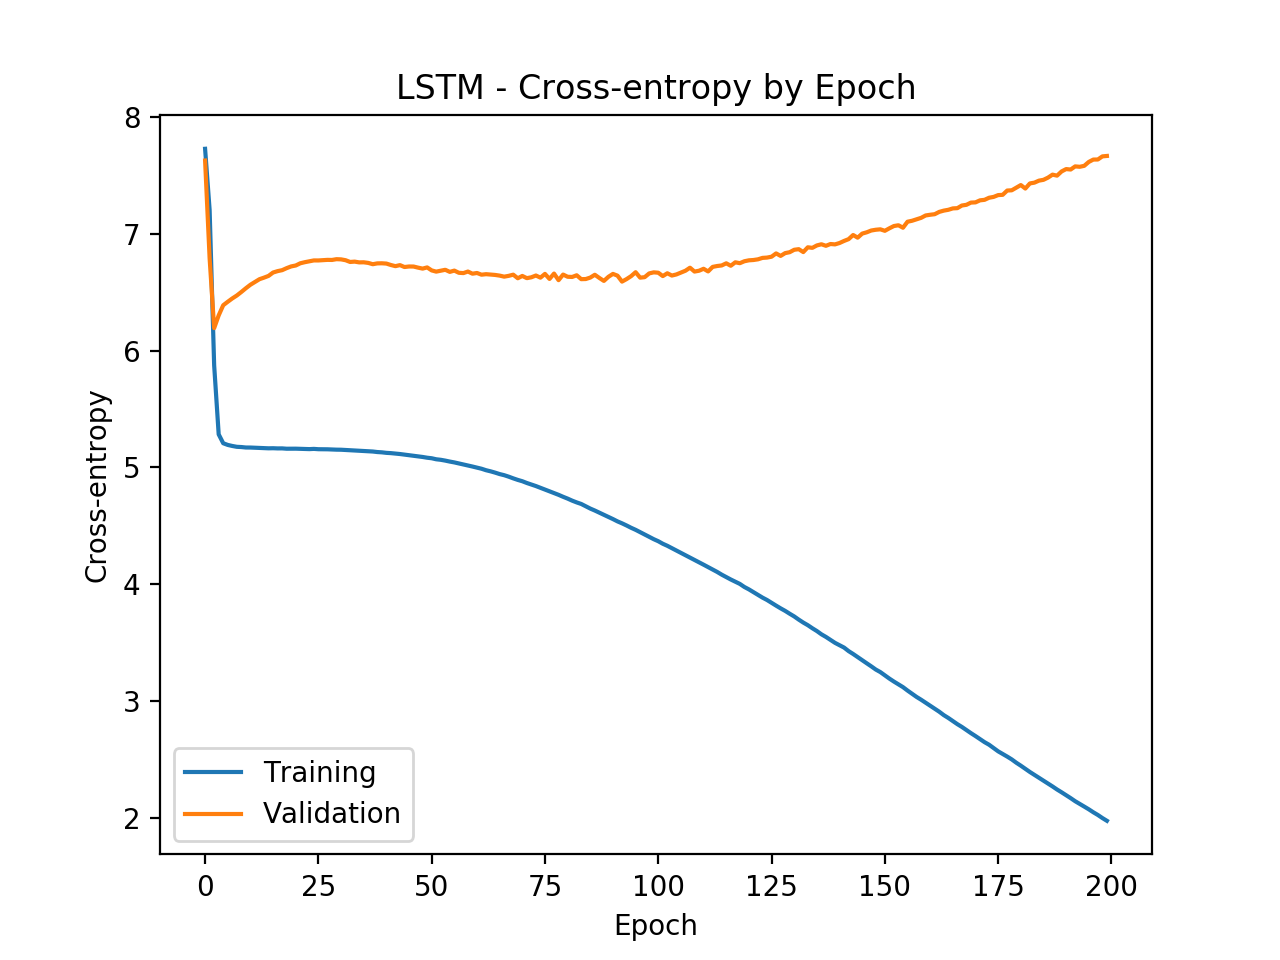
\includegraphics[width=0.42\textwidth]{LSTM_Loss.png}
    \caption{LSTM learning curves}
    \label{fig:LearningCurves}
\end{figure}


\subsubsection{Markov Chain Models}
\label{sec:markov}

The first Markov model is a trigram model with beam search. The sentences are processed backwards, using a bigram consisting of the seed word and an end-of-sentence token as input and stopping generation when a beginning-of-sentence token is predicted. An advantage of this model is the flexibility of the search function, which could be modified in future work to decrease the effects of data sparsity. However, despite its strong results, it was not included in final results due to overfitting concerns; given little data, it is likely to produce similar outputs to the text itself, especially with less common seed words. 

Given the difficulties in training a successful neural generator with small input data, and the concerns over overfitting the trigram model to the data, a third model based on an open-source implementation of a Markov chain model was used. A Markov chain is a statistical model which computes probabilities of sequences of variables from a set of possible values \cite[Chapter~8]{jurafskymarkov}. Figure \ref{fig:markov} shows a graphic of a Markov chain for word transitions.

\begin{figure}
	\centering
	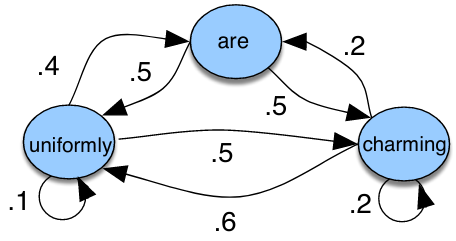
\includegraphics[scale=0.35]{./markov_chain.png}
	\caption{Markov chain for word transition probabilities \cite{jurafskymarkov}}
\label{fig:markov}
\end{figure}

The Markov chain implementation in the open-source \textit{markovify} \cite{markovify} library takes a text corpus as an input, splits it into sentences, and builds probabilities of forward word transitions starting from the beginning of each sentence and moving towards the end. New sentences are generated from a provided beginning word using word transitions observed in the input corpus.

Additional work was done by \citet{markovifyfork} to implement a backwards Markov chain generator. This reverses the order in which sentences from the corpus are consumed to build the model, resulting in word transitions that move backwards in a sentence starting from an ending word, suitable for the purposes of \textit{prose2poetry}.

%%%%%%%%%%%%%%
% EXP & RESULTS		%
%%%%%%%%%%%%%%
\section{Results}
\label{sec:results}

\subsection{Baseline Corpora}
\label{sec:corpora}

Using a similar approach to \citet{cole}, the Gutenberg Poetry \cite{gutenbergpoetry} and PoetryFoundation \cite{poetryfoundationkaggle} datasets were filtered to produce rhyming couplets. The filtering process uses the rhymes function available in the pronouncingpy library to extract every pair with rhyming end words from the same poem as a couplet. The total is 331,713 rhyming couplets from Gutenberg, and 10,009 rhyming couplets from PoetryFoundation.

\subsection{Couplet Evaluation}
\label{sec:coupleteval}

A couplet scoring function was developed to evaluate the couplets, consisting of two components -- the end word rhyme score, and a stress score which measures syllabic meter \cite{meter_def}.

\subsubsection{Rhyme Score}
\label{sec:rhymescore}

The rhyme score returns a real value representing the strength of the rhyme between two words. It uses phoneme data from the CMUdict in a mean of three heuristic scores:
\begin{tight_itemize}
	\vspace{-0.5em}
	\item \textit{Reverse consecutive phoneme matching} (RCPM):
	RCPM counts, in reverse order starting from the end of both words, how many consecutive phoneme matches occur between the two words, normalized by the maximum possible matches.
	\item \textit{Overall phoneme matching} (OPM):
		OPM counts all common phonemes between a pair of words without considering order. It's essentialy an adapted \citet{ratcliff} string similarity score, using phonemes instead of characters.
	\item \textit{Syllable count matching} (SCM):
	SCM is a ratio of the syllable counts. There is a subtraction by one in the numerator and denominator to allow the SCM to be zero in the worst case.
\end{tight_itemize}

These are combined in an evenly weighted average $\in [0, 1]$, illustrated in figure \ref{fig:rhymescore}. There are some additions for special cases:
\begin{tight_enumerate}
	\vspace{-0.5em}
	\item
		Identical words have a rhyme score of 0.
	\item
		Longer rhymes score higher, up to a ceiling of 6 phonemes. Without this, single-syllable words tend to dominate the rhyme score.
	\item
		If there are multiple possible pronunciations, rhyme score returns the maximum score across all the pronunciation permutations for both words, discussed further in section \ref{sec:synset}.
\end{tight_enumerate}

\begin{figure}[h]
    \centering
    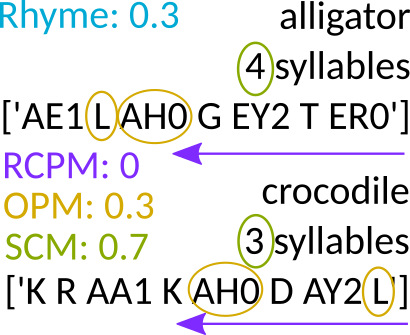
\includegraphics[scale=0.45]{rhyme_score.png}
    \caption{Rhyme score for \textit{alligator} and \textit{crocodile}}
    \label{fig:rhymescore}
\end{figure}

\subsubsection{Meter Score}
\label{sec:stressscore}

Using the pronouncingpy library, the syllabic stress of all of the words in each line is concatenated to represent the syllabic meter \cite{meter_def} of each sentence. In the CMUdict, 0 represents an unstressed syllable, 1 represents primary stress, and 2 represents secondary stress.  Examples are shown in table \ref{table:stress}. The \citet{ratcliff} string similarity score is then applied on the concatenated stress strings of the two sentences in the couplet.

\begin{table}
\centering
\begin{tabular}{ll c c}
	\hline\hline
	Sentence & Stress \\ [0.5ex]
	\hline\hline
	He likes jam & 111 \\ [0.5ex]
	\hline
	She likes ham & 111 \\ [0.5ex]
	\hline
	Alexander the Great conquered & 20100110 \\ [0.5ex]
	\hline
\end{tabular}
\caption{Cases of matched and mismatched stress strings for comparing meter}
\label{table:stress}
\end{table}

\subsubsection{Couplet Score}
\label{sec:coupletscore}

The total couplet score is the mean of rhyme and meter score, resulting in a single real value $\in [0, 1]$.
 The couplet score evaluates form only, and not contents. This can be problematic -- consider the example ``ham ham ham, jam jam jam.'' This couplet has a nearly perfect score of 0.89, but a human judge would (probably) not rate it as good poetry. There were many challenges involved in evaluating the semantic coherence, grammatical correctness, or other aspects of the contents of the couplets. These are discussed in section \ref{sec:nlg}.

\begin{table*}[ht]
\begin{tabular}{|l|l|l|l|l|l|l|l|l|l|l|c|c|c|c|c|c|c|c|c|c|}
\hline\hline
\multicolumn{1}{|c|}{Score} & \multicolumn{3}{c|}{Couplet} & \multicolumn{3}{c|}{Rhyme} & \multicolumn{3}{c|}{Meter}\\
\cline{1-10}
\multicolumn{1}{|c|}{Dataset} & Mean & SD & .95q & Mean & SD & .95q & Mean & SD & .95q \\
\hline\hline
Gutenberg & 0.69 & 0.12 & 0.86 & 0.70 & 0.18 & 0.93 & 0.68 & 0.14 & 0.89 \\ [0.5ex]
\hline
PoetryFoundation & 0.69 & 0.12 & 0.85 & 0.70 & 0.19 & 0.93 & 0.68 & 0.14 & 0.89 \\ [0.5ex]
\hline
\textbf{\textit{prose2poetry} LSTM} & \textbf{0.63} & \textbf{0.12} & \textbf{0.82} & \textbf{0.68} & \textbf{0.16} & \textbf{0.91} & \textbf{0.58} & \textbf{0.18} & \textbf{0.88} \\ [0.5ex]
\hline
\textbf{\textit{prose2poetry} Markov chain} & \textbf{0.57} & \textbf{0.13} & \textbf{0.77} & \textbf{0.68} & \textbf{0.16} & \textbf{0.90} & \textbf{0.47} & \textbf{0.19} & \textbf{0.76} \\ [0.5ex]
\hline
Prose & 0.34 & 0.13 & 0.56 & 0.19 & 0.18 & 0.46 & 0.48 & 0.19 & 0.76 \\ [0.5ex]
\hline
\end{tabular}

\caption{Couplet Scores of \textit{prose2poetry} Generated Outputs and Baselines}
\label{table:couplet_results}
\end{table*}

\begin{table*}[ht]
\begin{tabular*}{\textwidth}{ll cc}
	\hline\hline
	Source & Couplet \\ [0.5ex]
	\hline\hline
	Gutenberg baseline & (`Driven from his ancestral streams', `By the might of evil dreams') \\ [0.5ex]
	\hline
	PoetryFoundation baseline & (`Poets hate to have directives', `They’re on their own, not on collectives') \\ [0.5ex]
	\hline
	\textbf{\textit{prose2poetry} LSTM} & \textbf{(`as that he had so note', `was been now turned wrote')} \\ [0.5ex]
	\hline
	\textbf{\textit{prose2poetry} Markov chain} & \textbf{(`And how tired you must not propose', `Mr . Knightley could not oppose')} \\ [0.5ex]
	\hline
	Prose & (`i thought you meant to go with me', `they would be very much pleased') \\ [0.5ex]
	\hline
\end{tabular*}
\caption{Examples of top-scoring couplets from all evaluated datasets}
\label{table:bestcouplets}
\end{table*}

\subsection{Quantitative Assessment}

The results in table \ref{table:couplet_results} were evaluated on 1,000 couplets randomly selected from the baselines and \textit{prose2poetry} generator models. The evaluation was repeated with different RNG seeds, observing that different random selections of couplets from the same source tended to have a stable score.

The input corpus was \textit{Emma} by Jane Austen, and the seed words for both the LSTM and Markov chain generators were the following: love, hate, pride, prejudice, justice, romance. The prose baseline was created by selecting consecutive sentence pairs from the input corpus without filtering.

The total couplet score is shown, as well as each of the subcomponents for further discussion. The mean, standard deviation, and .95 quantile were chosen as statistical metrics.

\subsection{Qualitative Assessment}

From each evaluated dataset, one couplet which scored better than the .95 quantile score is included in table \ref{table:bestcouplets} for the readers to enjoy.

%%%%%%%%%%%%%%
% DISC & CONC		%
%%%%%%%%%%%%%%
\section{Discussion and Conclusion}
\label{sec:discconc}

The results of the couplet score in table \ref{table:couplet_results} were as anticipated in the hypothesis. The generated couplets scored better than couplets from the prose corpus, but lower than real poetry. The main contributor of this difference is the meter score, which is significantly lower for the generated couplets. This was expected, as meter was not enforced in either model.

In terms of variability in the results, the generated sentences have a more stable rhyme score than the human poetry. This indicates that human poets don't necessarily consider perfect end rhymes as a requirement. The inverse was true for meter, where human poetry scores stably higher. This confirms that syllabic meter is an important device in human poetry. In future work, meter could be incorporated in the generator models.

\subsection{Generated Sentence Semantic Relatedness}
\label{sec:doc2vec}

As explained in section \ref{sec:fasttext}, the word pairs were selected to be related in context in the hopes that the two resulting generated sentences would be semantically related as well. An analysis was conducted to validate this assumption with the \textit{doc2vec} sentence embedding \cite{docvec}. The hyperparameters were shown in table \ref{table:HP_fasttext}, and it was trained on the same input corpus.

For the Markov chain model, the cosine distance between the embedding vectors of two generated sentences showed an improvement of 10\% (evaluated across 1,000 generated couplets) when using end words that had a high \textit{FastText} cosine distance, justifying the design of word pair generation. However, the LSTM model only improved by 0.6\%.

% Markov: 0.51799 vs 0.562932 
% LSTM: 0.607907 vs 0.611643

\subsection{LSTM Model Discussion}
\label{sec:discconclstm}

The trained LSTM described in section \ref{sec:lstm} did not perform to the expected standard. Using additional input corpora would go against the spirit of \textit{prose2poetry}, so it was discarded as an option. One possible alternative could have been to use a pre-trained language model such as GPT-2 \cite{gpt2}, fine-tuned with the input corpus.

\subsection{Homograph Sense Disambiguation}
\label{sec:synset}

Associating different pronunciations of homographs with their respective senses or parts of speech proved difficult, a problem also noted by \citet{hopkins-kiela-2017}. Consider an example, using WordNet \cite{wordnet} as a lexical resource. There are two pronunciations for ``bow'' in the CMUdict: like ``cow'' or like ``snow''. In WordNet, there are fourteen synsets for ``bow'', and two different parts of speech.

There is no readily available mapping between CMUdict pronunciation and WordNet senses. This can only be resolved with a lexical resource that provides combined sense and pronunciation disambiguation -- Wiktionary \cite{wiktionary} is one such option, but scraping it was considered beyond the scope of this paper. The final approach chosen was to ignore ambiguity and return the best rhyme score across all pronunciation permutations.

\subsection{Sentence Content Evaluation}
\label{sec:nlg}

The biggest difficulty encountered in \textit{prose2poetry} was in quantitatively evaluating the contents of the couplet. Sentence correctness is especially tricky with poetry, which does not necessarily need to strictly obey grammar. The field of NLG evaluation was explored for ideas to evaluate correctness. \citet{nlgeval} present a survey on popular automated metrics for evaluating machine-generated text in several applications including machine translation. They found that METEOR \cite{meteor} correlates well at the sentence level with human judgement.

A requirement of automated NLG evaluation metrics is reference sentences to compare the inputs to. It is unclear what these should be when evaluating poetry. In an early experiment, the baseline Gutenberg poetry corpus was used as reference sentences in METEOR, hoping this would assign high scores to good poetry. This did not provide any meaningful results, and NLG metrics were deemed inappropriate for evaluating couplets.

\subsection{Code Availability}

The Python code for \textit{prose2poetry} is on GitHub\footnote{\href{https://github.com/milhouse74/prose2poetry}{https://github.com/milhouse74/prose2poetry}}.

%%%%%%%%%%%%%%
% STAT OF CONT		%
%%%%%%%%%%%%%%
\section{Statement of contributions}
\label{sec:contributions}
Sevag found and prepared the datasets, created the code architecture, implemented the couplet score and third-party Markov chain generator, and ran the evaluations. François developed the vector embedding models (FastText and doc2vec), the word pair generation, the LSTM generator, and the rhyme score. Sophie discovered the pronunciation-sense ambiguity problem and wrote the initial prototype Markov chain generator.

\vfill
\clearpage % force a page break before references

\bibliographystyle{acl_natbib}
\bibliography{final_report}

\end{document}
